\chapter{Implémentation}

\section{Architecture physique et interfaces}

Grâce à l'architecture physique (cf figure \ref{fig:archiPhysique}), nous avons pu déduire que notre projet se décomposait en trois sous-systèmes : les interfaces d'acquisition, logicielle et graphique.

\begin{figure}[H]
  \centering
  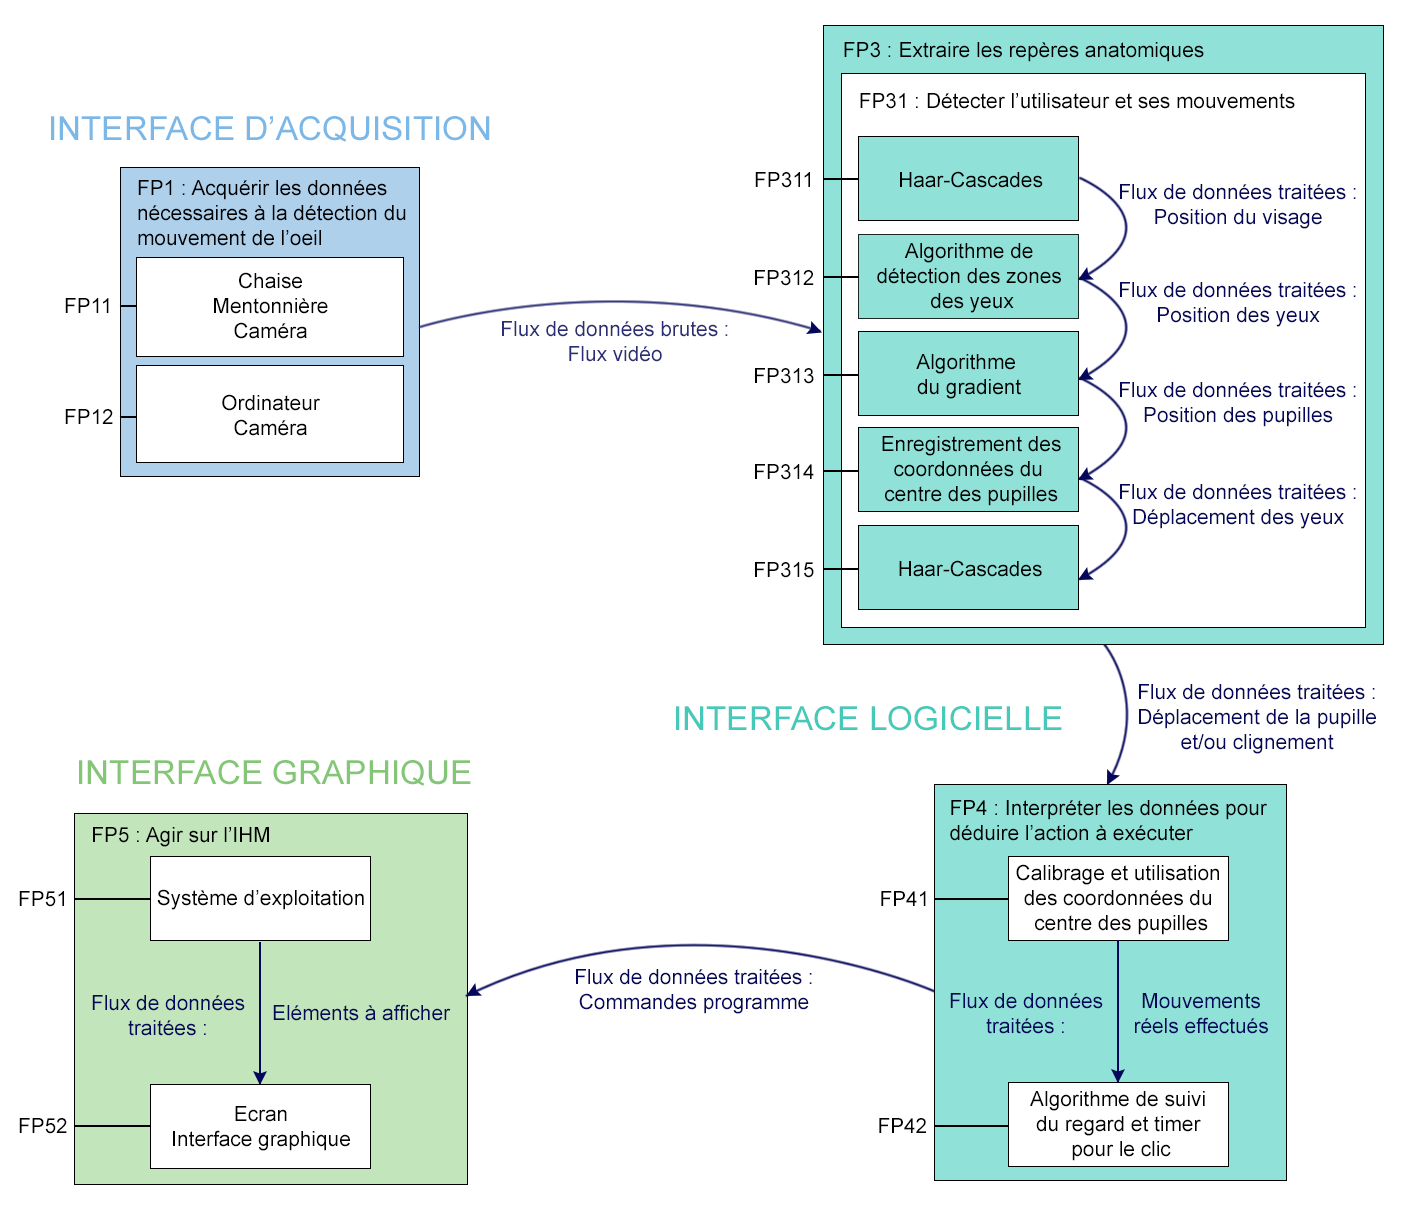
\includegraphics[scale=1.2]{architecturePhysique}
  \caption{Architecture Physique}
  \label{fig:archiPhysique}
\end{figure}

\subsection{Interface d'acquisition}
Cette interface est constituée principalement de la caméra et de la mentonnière. Cette dernière est utilisée pour éviter les mouvements de la tête, non traités par le programme. L'ordinateur occupe également une place secondaire, puisqu'il permet de vérifier que l'utilisateur est convenablement installé.

\subsection{Interface logicielle}
L'interface logicielle s'appuie sur le programme contenant des algorithmes développés en C++ avec OpenCV. Ils ont pour but de traiter les images transmises par la webcam afin de détecter le visage, puis les yeux et enfin les pupilles et les clignements pour déduire l'action que l'utilisateur souhaite effectuer. Que ce soit pour le clic ou le mouvement du curseur de la souris, une interaction avec l'OS est nécessaire. Le programme doit donc être adapté suivant le système d'exploitation utilisé.

\subsection{Interface graphique}
Enfin, le rôle de l'interface graphique est de proposer à l'utilisateur un choix de boutons qui lancent des applications. Cette dernière est développée en C++ à l'aide de Qt Creator et ne peut être utilisée que sur Windows car il faudrait changer toutes les commandes d'ouverture d'applications pour exécuter le programme sur un autre système d'exploitation.

\section{WBS}
La structure de découpage du projet découle de l'architecture physique. La figure \ref{fig:WBS} illustre le WBS ainsi établit. 

\begin{figure}[H]
  \centering
  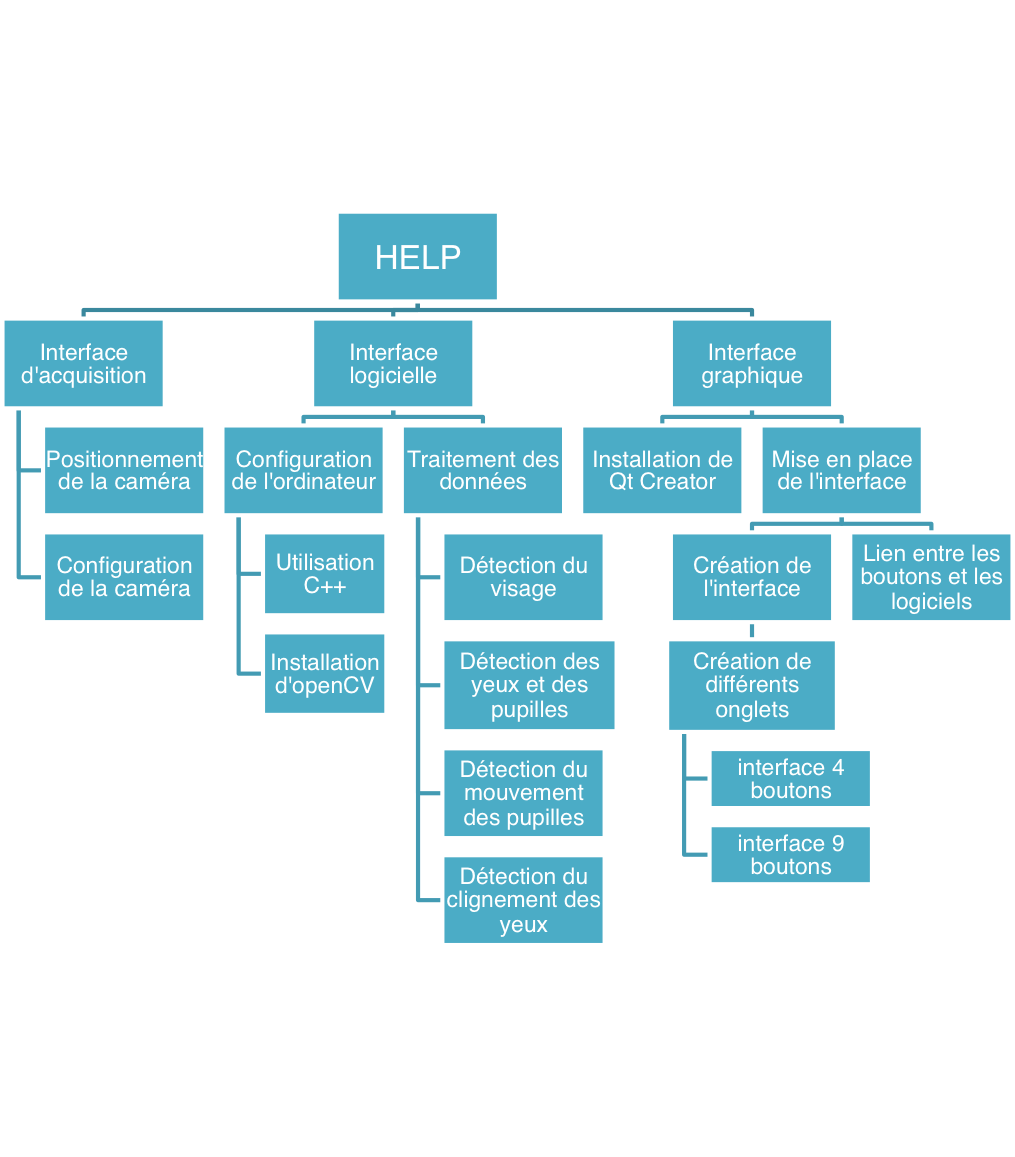
\includegraphics[scale=0.8]{WBS}
  \caption{WBS}
  \label{fig:WBS}
\end{figure}